\documentclass{article}

\usepackage[english]{babel}
\usepackage[utf8x]{inputenc}
\usepackage[T1]{fontenc}
\usepackage[]{physics}
\usepackage{amsmath}
\usepackage{natbib}
\usepackage{hyperref}
\usepackage{appendix}
\usepackage{caption}
\usepackage{enumitem}
\usepackage{mathtools}
\hypersetup{colorlinks=false, linkcolor=black,}

%% Sets page size and margins
\usepackage[a4paper,top=3cm,bottom=2cm,left=3cm,right=3cm,marginparwidth=1.75cm]{geometry}

%% Useful packages
\usepackage{amsmath}
\usepackage{graphicx}
\usepackage{subfiles}
\renewcommand{\baselinestretch}{1}
\setlength{\parskip}{1em}
\setlength{\parindent}{0pt}

\title{Short Term Prediction of State of Charge for Commercial Electric Vehicles}
\author{Angus Campbell}
\date{June 2019}

\begin{document}

\maketitle
\tableofcontents

\newpage
\begin{abstract}
    
\end{abstract}

\section{Introduction}

% - Why EV's are now important in the context of the predicted future uptake and tackling GHG's.

% - Current problems facing electric vehicles e.g. Why knowing and predicting SoC is important and the barriers facing it, costs associated with this like constructing charging infrastructure and scheduling.

% - EV fleet charging management require accurate models at predicitng energy demand which is based off SoC at destination. 

% - Specifically the problems facing commercial EV's and public transport EV's.

% - Previous tests using lab tested/ simulated data for the preformance of batteries in EV's.

% - What this paper is proposing.

A global shift from traditional fossil fuel powered vehicles to battery powered electric vehicles (EV's) has been identified as one of the key cornerstones of a decarbonised future. 
\begin{itemize}
    \item What are the current standards for prediction of real world consumption for commercial EV's?
    \item What are the limitations for current models for commercial EV's?
    \item Quantify the specific effects from various factors upon the the energy consumption for the fleet of electric buses and ascertain which are most useful; in modelling electric bus consumption.
    \item Provide a model for the forecasting of Energy Demand using methods selected from literature with the aim of creating a framework which tests forecasting for various time lengths into the future.
    \item Use the insights gained from exploratory analysis and modelling of SoC to: provide suggestions for the scheduling of the electric fleet/ discuss the feasibility and uptake of new services on more routes.
\end{itemize}

\section{Literature Review}

As discussed in the previous section the growing share of the total vehicle population has slowly led to an increase in the literature using models from real world data to estimate range or consumption for EV's. The increased use of this data presents its own unique problems including a lack of sufficient data for more complex models \citep{Yang2017} or quantifying the variation due to specific variables that have significant interactions \citep{Liu2018}. 


\subsection{Battery Degradation}

\subsubsection{State of Charge and Capacity}

 
\begin{equation}\label{eq:1}
    SoH = \frac{Q_{measured}}{Q_{rated}}
\end{equation}


\begin{table}[ht]
\centering
\begin{tabular}{rlrr}
  \hline
 & Variable & Missing Values & \% of Total Values \\ 
  \hline
1 & Analysis - soc - SOC used [\%] & 894046 & 78 \\ 
  2 & Analysis - soc - SOC used per day [\%] & 892979 & 78 \\ 
  3 & Engine - Engine RPM [rpm] & 879085 & 77 \\ 
  4 & Analysis - energy - Energy charged per day [kWh] & 819778 & 71 \\ 
  5 & DC/DC - Controller temp [°C] & 791114 & 69 \\ 
  6 & Battery - State of Charge [\%] & 732071 & 64 \\ 
  7 & Analysis - energy - Energy consumed per day [kWh] & 694165 & 60 \\ 
  8 & Dashboard - Speed [mph] & 678607 & 59 \\ 
  9 & Battery - Battery voltage [V] & 619897 & 54 \\ 
  10 & Battery - Battery current [A] & 596763 & 52 \\ 
  11 & Battery 1 - Voltage [V] & 522248 & 45 \\ 
  12 & Battery 1 - Current [A] & 513352 & 45 \\ 
  13 & Battery 1 - State of Charge [\%] & 498687 & 43 \\ 
  14 & GPS - GPS position Latitude & 303604 & 26 \\ 
  15 & GPS - GPS position Longitude & 303604 & 26 \\ 
  16 & GPS - Altitude [m] & 272212 & 24 \\ 
   \hline
\end{tabular}
\caption{Sample of data provided by Arriva.}
\label{table:1}
\end{table}

As shown by the proportion of missing values in the table the data provided had many sparse variables. Due to the high percentages of missing values many variables would have proven difficult to interpolate and so the decision was taken to simply remove the missing values form key variables which were: GPS positions and Dashboard Speed. As SoC and energy consumed within a day were ongoing counts of the buses state, an assumption was made that the sparsity of these variables was at an acceptable level and more value would be gained from keeping the information provided by the other variables for the specific row entries.

After the missing values were removed from the data, outliers and extreme values were also removed from the data set. To remove such variables the mean ($\mu$) and standard deviation ($\sigma$) for variables 1 to 13 (see table \ref{table:1}) were first calculated. The upper and lower limit were specified as $\mu \pm 3\sigma$ with any values exceeding this interval removed. These limits were chosen to incorporate 99.7\% of the data. However some variables still require additional "common sense" limits such as the SoC not exceeding 100\% and the energy consumed per day being a non-negative value (outside of charging).

\subsection{Weather Data}

Weather data was collected from between June 2016 and May 2019 along the 312 route. The data was collected using the freely available Dark Sky API. The data was collected at hour resolution using GPS coordinates for the centre of the bus route. A summary of the data collected from Dark Sky is given in table \ref{table:weather} below.

\begin{table}[h!]
\centering
\begin{tabular}{rlrrrrrrrr}
  \hline
 & Variable & count & mean & std & min & X25. & X50. & X75. & max \\ 
  \hline
1 & precipProbability & 13554.00 & 0.13 & 0.23 & 0.00 & 0.00 & 0.02 & 0.14 & 0.82 \\ 
  2 & temperature & 13554.00 & 62.15 & 7.37 & 47.26 & 56.64 & 62.49 & 66.19 & 89.84 \\ 
  3 & apparentTemperature & 13554.00 & 62.17 & 7.48 & 45.68 & 56.64 & 62.51 & 66.47 & 89.84 \\ 
  4 & dewPoint & 13554.00 & 52.23 & 5.63 & 38.14 & 48.76 & 51.15 & 55.93 & 65.70 \\ 
  5 & humidity & 13554.00 & 0.72 & 0.16 & 0.32 & 0.59 & 0.74 & 0.85 & 1.00 \\ 
  6 & pressure & 13554.00 & 1014.82 & 6.76 & 997.88 & 1010.57 & 1014.06 & 1019.18 & 1029.33 \\ 
  7 & windSpeed & 13554.00 & 9.93 & 4.00 & 0.75 & 6.92 & 9.72 & 13.02 & 21.04 \\ 
  8 & windGust & 13554.00 & 16.64 & 7.36 & 2.23 & 10.28 & 15.91 & 22.13 & 35.95 \\ 
  9 & windBearing & 13554.00 & 176.03 & 86.81 & 2.00 & 92.00 & 200.00 & 238.00 & 358.00 \\ 
  10 & cloudCover & 13554.00 & 0.53 & 0.26 & 0.00 & 0.36 & 0.52 & 0.75 & 1.00 \\ 
  11 & uvIndex & 13554.00 & 2.62 & 2.14 & 0.00 & 1.00 & 3.00 & 4.00 & 8.00 \\ 
  12 & visibility & 13554.00 & 6.09 & 0.85 & 0.01 & 6.02 & 6.22 & 6.22 & 10.00 \\ 
   \hline
\end{tabular}
\caption{A summary table of the weather variables obtained from Dark Sky API.}
\label{table:weather}
\end{table}


%Explain further when talking through parts of the filter?
%Need to define journey as a trip without charging?

\begin{figure}[ht]
    \centering
    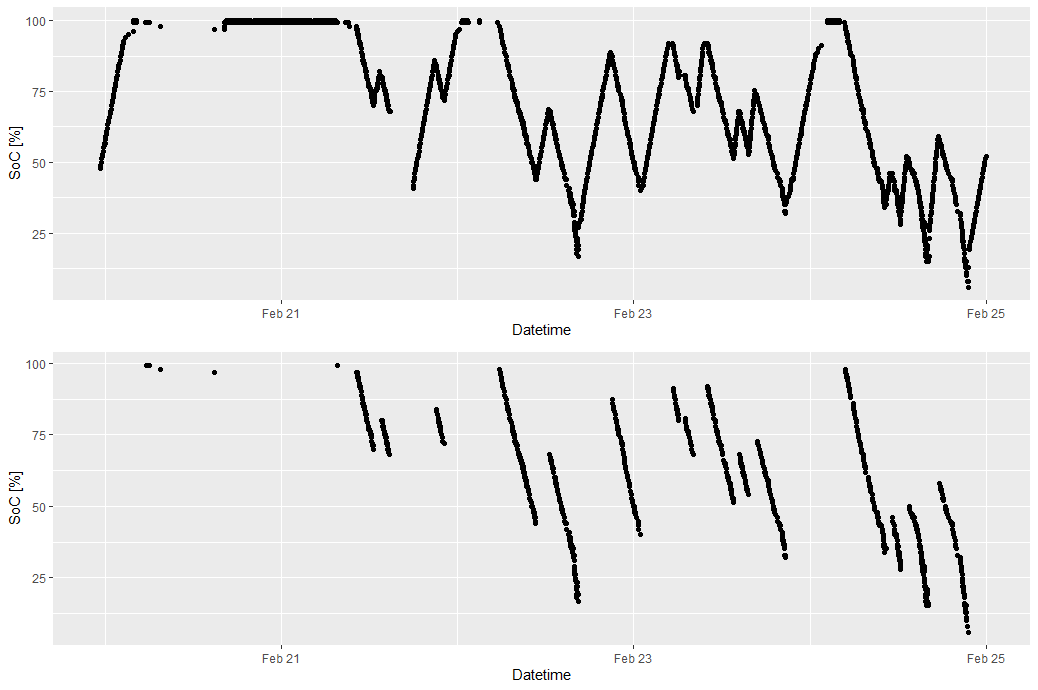
\includegraphics[width = 0.8\textwidth]{Raw_and_unflitered_SoC_EMC_3_2018.png}
    \caption{Plots showing the SoC percentage over time for a single bus over a small sample of days in 2018. The top plot is the raw uncleaned data including charging events and longer periods in which the bus was found to be stationary. The bottom plot shows just the SoC during bus journeys from the cleaned dataset.}
    \label{fig:2}
\end{figure}

% Need to align the axes properly, potnetially add the resutls to the same df
%is just a plot of SoC over time enough or is a quick test needed to prove more rigorously that it follows a linear 

Again as shown in figure \ref{fig:2} a single bus will generally conduct between 0-4 journeys between charging instances per day often of varying lengths of time and therefore varying proportions of SoC are used. The algorithms proposed are in the form of two filters aimed to extract to the two longest journeys undertaken by a singular bus on a certain date. The process for the two filters is outlined within the figures below.

\begin{figure}[ht]
    \centering
    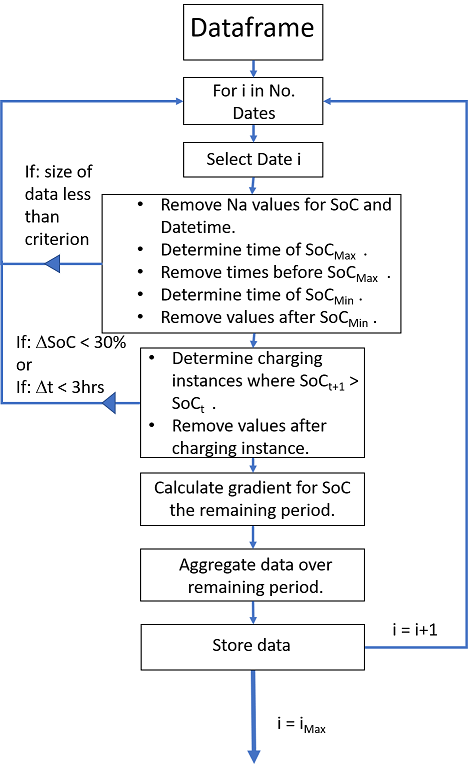
\includegraphics[width = 0.5\textwidth]{Filter_1_powerpoint.png}
    \caption{Sketch of filter 1 to be redone.}
    \label{fig:3}
\end{figure}


\begin{equation}
\begin{split}
\frac{d}{dt}(SoC)  & = \beta_1*t + \beta_2*SoC_{Start} + \beta_3*(wind direction) + \beta_{4}*(wind speed) + \beta_{5}*(wind bearing) \\ 
& + \beta_{6}*d + \beta_{7}* speed_{kmh} + \beta_{8}*V*I + \beta_{9}*Bus_{id} +         \beta_{8}*T(^oC) + \beta_{10}*a + \beta_{11}*CMF + \\ 
& \beta_{12}*\Delta h + \beta_{13}*Wday + \beta_{14}*Month + \beta_{15}*Year + \beta_{16}*hour_{SoC_{Max}} + \epsilon 
\label{eq:7}
\end{split}
\end{equation}

\noindent Where
\begin{description}[labelindent=10pt,labelsep=10pt]
\item[$t$] : length of time for the journey in seconds 
\item $SoC_{Start}$ : The starting SoC of the Vehicle 
\item $wind direction$ : The projection of the wind bearing on the the direction on the vehicle
\item $d$ : The total distance traveled (km)
\item $V$ : The mean voltage across the battery for the journey 
\item $I$ : The mean current across the battery for the journey 
\item $Bus_{id}$ : The specific vehicle 
\item $T(^oC)$ : Ambient temperature $(^oC)$ 
\item $a$ : The mean acceleration of the vehicle 
\item $CMF$ : The total Constant motion factor  of the journey 
\item $\Delta$ h: The total elevation gain by the vehicle 
\item $Wday$ : The day of the week
\item $hour_{Soc_{Max}}$ : The starting time of the journey 
\item $\epsilon$ : Error term
\end{description}

% Can use the fact that the observations are correlated as a reason to avoid this first section. 
% OLS assumptions need the observations to be uncorrelated which doesn't  really work with the minute by minute data. 
% OLS assumptions error is a random variable with mean 0, errors are uncorrelated (homoscedastic), no correlation between 
\newpage

\bibliographystyle{agsm}
\bibliography{Dissertation.bib}

\appendix
\section{Feature Generation}

\section{SoC Filter}
% EMC_! has all of it.

\section{Weather Correlation}

\begin{figure}[ht]
    \centering
    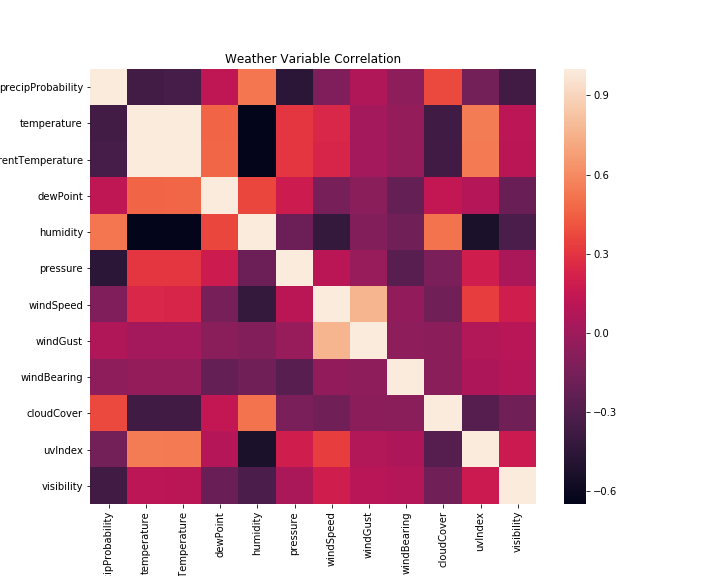
\includegraphics[width = \textwidth]{weather_correlation.png}
    \caption{Caption}
    \label{fig:weather_cor}
\end{figure}

\section{Filter results}

\begin{figure}
    \centering
    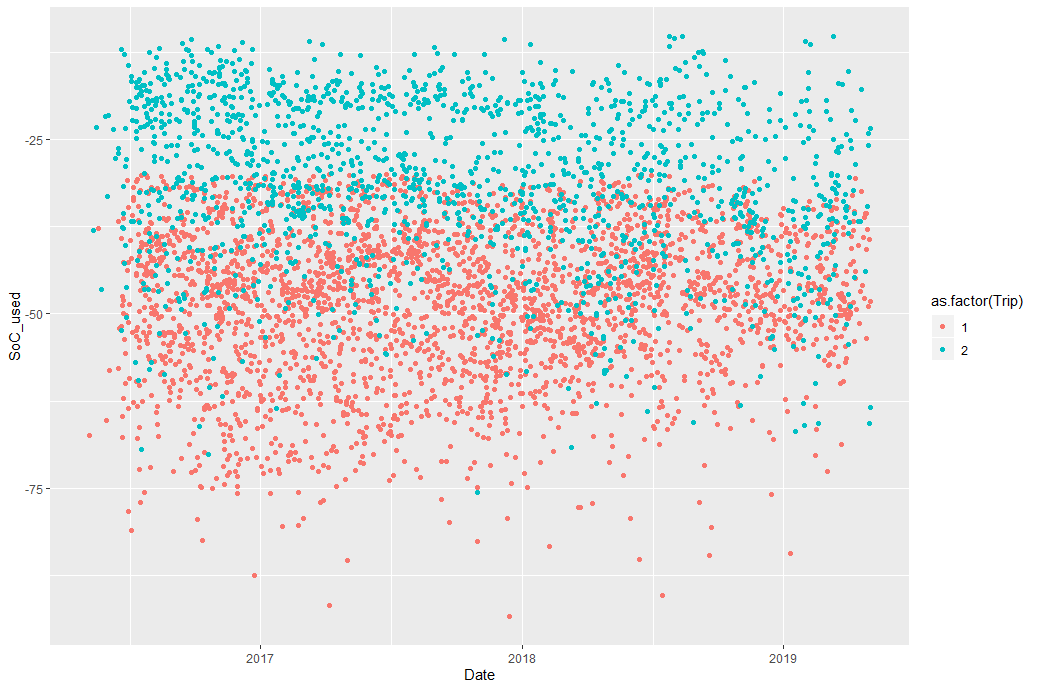
\includegraphics[width = \textwidth]{SoC_used_per_trip_by_filter.png}
    \caption{Caption}
    \label{fig:soc_per_trip}
\end{figure}

\begin{figure}
    \centering
    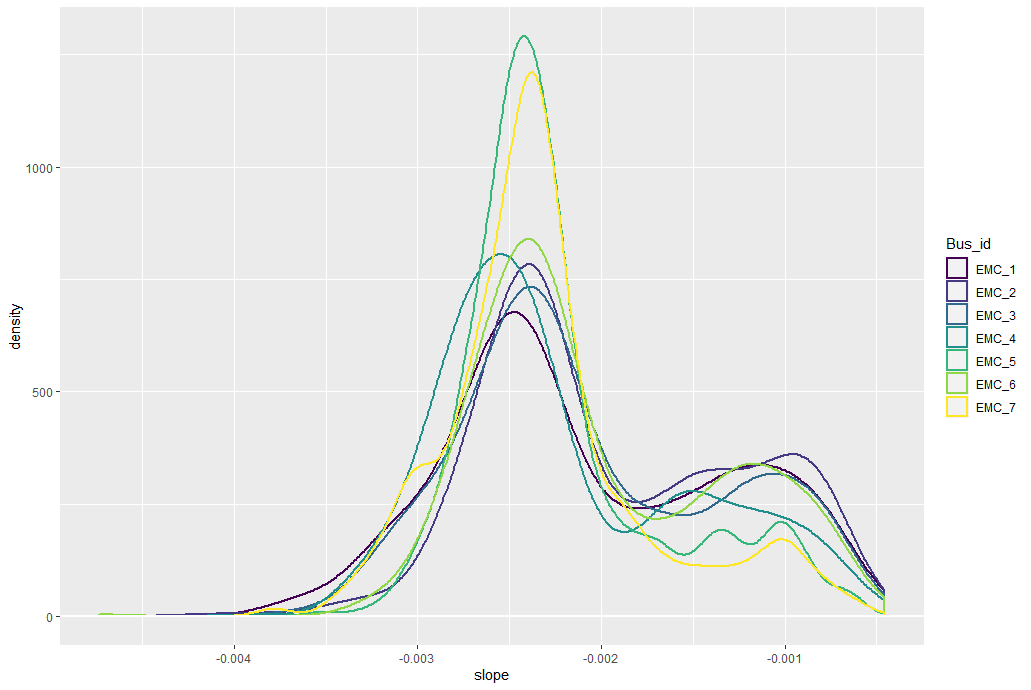
\includegraphics[width = \textwidth]{EMC_slopes.png}
    \caption{A plot showing the distribution of rates of decrease for SoC over the day for the individual buses in the fleet.}
    \label{fig:emc_slopes}
\end{figure}

\begin{figure}[h]
    \centering
    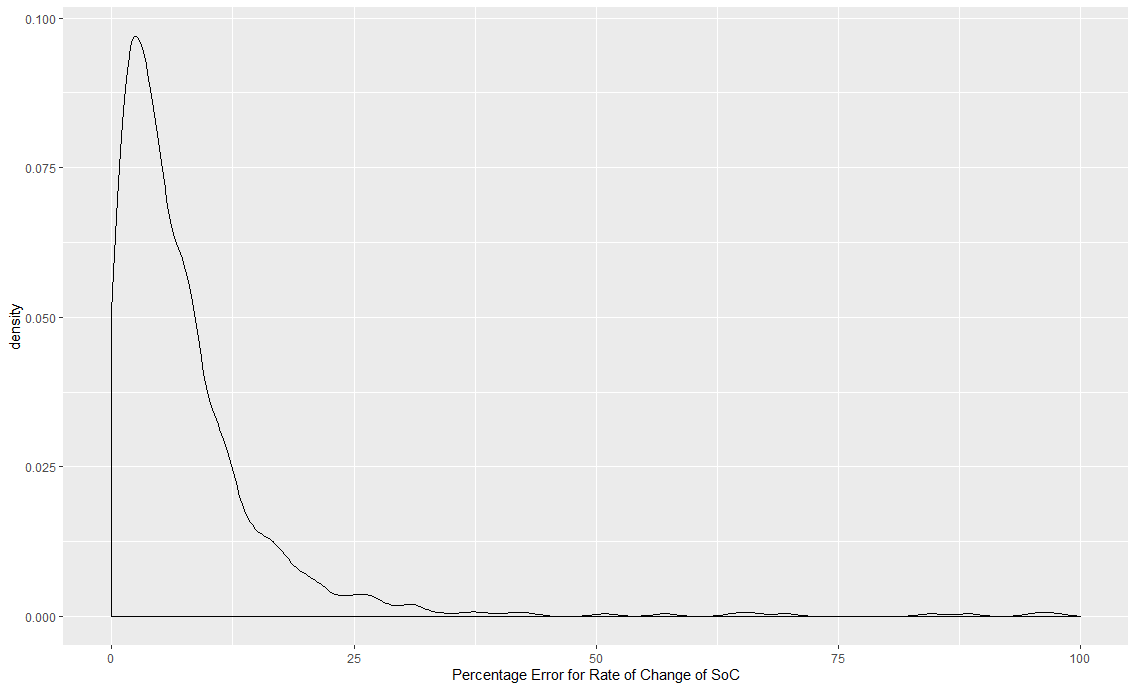
\includegraphics[width = 0.8\textwidth]{Percentage_error_density_model_4.png}
    \caption{The distribution of the percentage errors calculated for the first model using data from both filter 1 and filter 2.}
    \label{fig:9}
\end{figure}

\begin{figure}[h]
    \centering
    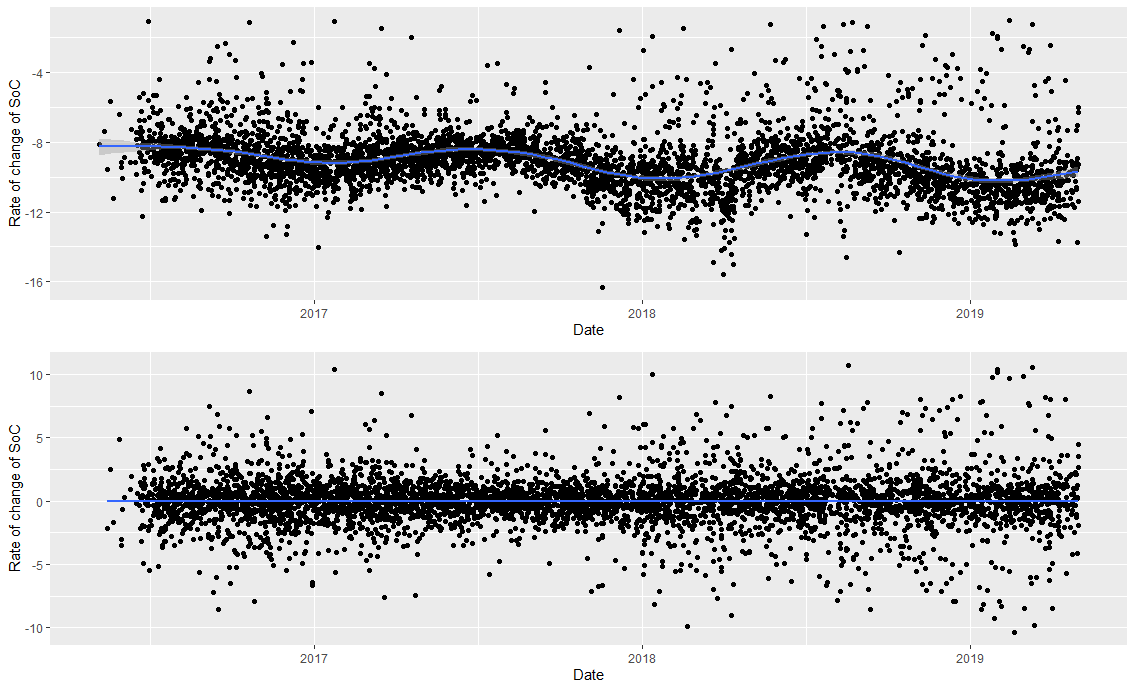
\includegraphics[width = 0.8\textwidth]{Sationary_transform.png}
    \caption{A plot of the non-stationary data vs the transformed stationary data. The transformation doesn't appear to add any clarity to the the model.}
    \label{fig:transform}
\end{figure}

\end{document}
